%%=============================================================================
%% Chaos Engineering Tools
%%=============================================================================

\chapter{\IfLanguageName{dutch}{Chaos Engineering Tools}{Chaos Engineering Tools}}
\label{ch:chaostools}

Het toepassen van chaos engineering is relatief nieuw, maar er zijn ondertussen al heel wat tools op de markt verschenen om chaos experimenten te kunnen uitvoeren. De Cloud Native Computing Foundation (CNCF), een Linux Foundation project gestart in 2015, is de thuisbasis van heel wat open source projecten die vandaag het landschap definiëren in de IT-sector. CNCF projecten kunnen drie niveaus van maturiteit hebben nl. sandbox, incubating en graduated. Deze niveau's geven aan hoe ver een project geëvolueerd is. \autocite{CNCF2022a}
\newline Men kan een overzicht van deze projecten, gerangschikt per categorie, terugvinden in het CNCF Cloud Native Interactive Landscape. Eén van deze categorieën is chaos engineering, waar men  een lijst kan terugvinden van chaos engineering tools. \autocite{CloudNativeLandscape2022}

Pavlos Ratis, Site Reliability Engineer bij RedHat OpenShift, onderhoudt een Github repository  waar men heel wat zaken omtrent chaos engineering kan terugvinden. In deze repository vindt men in de sectie 'Notable Tools' een lijst van chaos engineering tools die bruikbaar zijn voor verschillende doeleinden. Deze lijst werd eveneens geraadpleegd in de zoektocht naar een geschikte tool om chaos engineering experimenten toe te passen op een Kubernetes cluster. \autocite{Ratis2022}.

De eerste tool die onderzocht werd is Chaos Toolkit, via een cursus op het online leerplatform Udemy. Nadien kwamen uit de eerder vernoemde bronnen nog twee andere tools naar boven genaamd ChaosMesh en Litmus.

Vooraleer men experimenten kan beginnen uitvoeren heeft men eerst een demo-applicatie nodig. Volgend hoofdstuk beschrijft hoe men twee demo-applicaties kan opzetten waar men later experimenten op kan toepassen. Deze identieke setup zal gerepliceerd worden telkens een chaos engineering tool besproken wordt.

Daarna komt de installatie van de verschillende chaos engineering tools en het uitvoeren van de experimenten aan bod.

\section{Demo-applicaties opzetten}

 Aangezien dit onderzoek gericht is om experimenten uit te voeren voor educatieve doeleinden, is gekozen om eerst enkele experimenten uit te voeren op Nginx en Apache webserver pods. Door twee aparte Deployments en Services op te zetten kon de onderlinge communicatie tussen beiden aangetoond en getest worden. Dit was praktisch om experimenten uit te voeren waarbij de communicatie verstoord werd tussen verschillende Services, of experimenten enkel te richten op specifieke pods in een namespace. 

Het visuele aspect ontbrak hierbij echter om de impact van een experiment te verduidelijken op de applicatie in een browser. Vandaar is gekozen om enkele experimenten te herhalen op een tweede demo-applicatie genaamd PodTato-Head, een applicatie die een aardappelmannetje toont en waarbij de lichaamsdelen bestaan uit verschillende pods, opgezet via afzonderlijke Deployments en Services.   Met behulp van deze applicatie kon o.a. aangetoond worden dat een applicatie nog steeds bereikbaar kan zijn desondanks bepaalde pods getroffen worden.

\subsubsection{Demo-applicatie 1:Nginx/Apache webserver pods}

De eerste demo applicatie kan men onderbrengen in een aparte namespace genaamd demoapp1. Op deze manier kan men de impact van de experimenten (= de blast radius) beperken en voorkomen dat andere pods ongewenst mee betrokken worden in een experiment. Om de eerste demo-applicatie tot stand te brengen voert men volgende commando's uit: 
\begin{lstlisting}[language=bash]
    # Creëer een nieuwe namespace voor de experimenten
    $ kubectl create ns demoapp1
    
    # Creëer een Deployment met 3 Apache pods
    # in de namespace litmusexperiments
    $ kubectl create deploy apache --image=bitnami/apache \
    --replicas=3 -n demoapp1
    
    # Creëer een Deployment met 3 Nginx pods 
    # in de namespace demoapp1
    $ kubectl create deploy nginx --image=nginx \
    --replicas=3 -n demoapp1
    
    # Creëer een Service voor de Nginx pods
    $ kubectl expose deploy nginx --port=80 \
    -n demoapp1
    
    # Creëer een Service voor de Apache pods
    # Apache luistert in container op poort 8080
    $ kubectl expose deploy apache --port=80 \
    --target-port=8080 -n demoapp1           
\end{lstlisting} 

\subsection{Demo-applicatie 2: PodTato-Head}

De tweede demo applicatie PodTato-Head kan men onderbrengen in een aparte namespace genaamd demoapp2. De manier hoe deze geïnstalleerd wordt is opnieuw via het eerder gebruikte Helm, alhoewel men ook o.a. kubectl kan gebruiken om deze te installeren. \autocite{Gavant2022}

Maak eerst een nieuwe directory aan op het systeem waarin men in volgende stappen de PodTato-Head repository kan in bewaren. 

Men voert volgende commando's uit in de nieuwe directory om de applicatie te installeren:
\begin{lstlisting}[language=bash]
    # Creëer de namespace demoapp2
    $ kubectl create ns demoapp2
    
    # Kloon de podtato-head Git repo in de directory
    $ git clone https://github.com/podtato-head/podtato-head.git
    
    # Ga verder naar de podtato-head directory
    $ cd podtato-head/
    
    # Installeer de podtato-head app in namespace demoapp2
    $ helm install podtato-head ./delivery/chart -n demoapp2 
    
    # Verifieer als de app pods + services operationeel zijn
    $ kubectl get pods -n demoapp2
    $ kubectl get svc -n demoapp2
\end{lstlisting} 

Men kan de applicatie controleren in de browser door gebruik te maken van de info uit laatst vernoemde commando. Men kan zien dat bij de opgelijste Services 1 LoadBalancer geconfigureerd is, die de toegang van buitenaf tot de applicatie mogelijk maakt. Men kan in de browser het externe IP-adres van de LoadBalancer service gebruiken in combinatie met de poort 9000 waarop de applicatie actief is: {\bf http://[Loadbalancer-IP]:9000}. \newline Zie figuur \ref{img:podtato-head} als voorbeeld hoe de applicatie er in de browser uitziet. 

\begin{figure}[h]
    \centering
    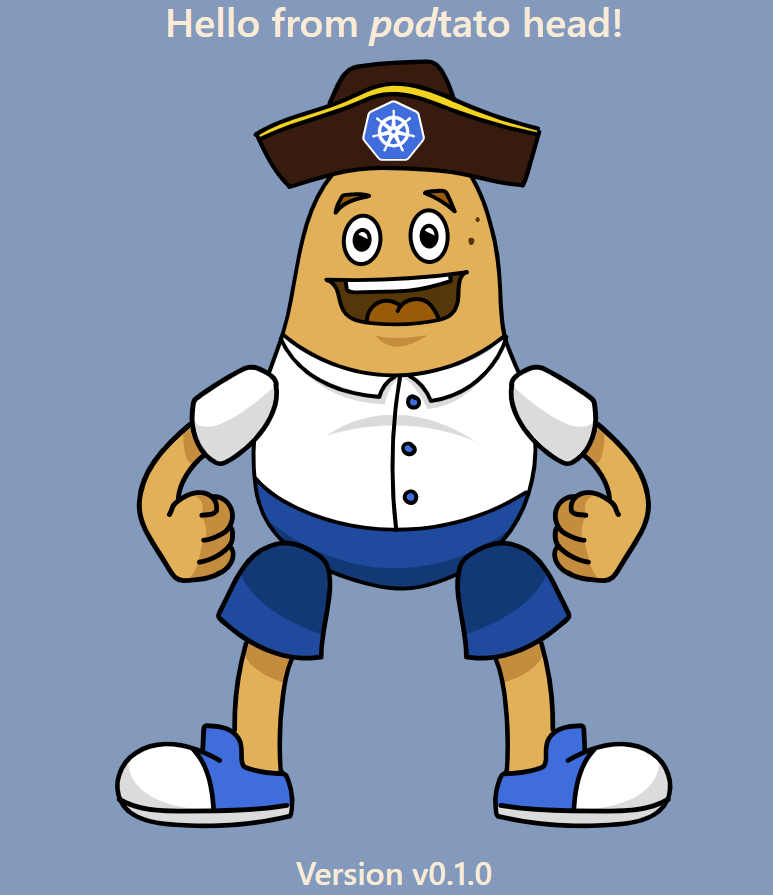
\includegraphics[scale=.5]{img/podtatohead-app.png}
    \caption{Podtato-Head applicatie}
    \label{img:podtato-head}
\end{figure}

Nota: Bovenstaande output bevat een LoadBalancer Service, maar in geval de applicatie in een lokale omgeving geïnstalleerd wordt zal hier een NodePort of ClusterIP te zien zijn. In dat geval zal men andere stappen moeten ondernemen om de toegang tot de applicatie in de browser te bekomen. 
Zie sectie {\bf Test the API Endpoint} in de bron die aan het begin van dit hoofdstuk vermeld wordt, waar de nodige acties omschreven worden om toe te passen in deze verschillende situaties.  

\section{Chaos Toolkit}

\section{Chaos Mesh}

\section{Litmus}

In de zoektocht naar een chaos engineering tool die net zoals voorgaande tool ChaosMesh zowel experimenten kon uitvoeren vanuit de terminal als via de browser, werd de keuze gemaakt om Litmus te onderzoeken. 

Het Litmus project startte in 2017 met als doel om simpele chaos experimenten op te zetten in een Kubernetes cluster. Het werd een Cloud Native Computing Foundation (CNCF) sandbox project in 2020, en wordt vandaag onderhouden door vijf verschillende organisaties. Sinds begin 2022 is het project geëvolueerd naar een CNCF incubating project. \autocite{CNCF2022}

\subsection {Vereisten}
\label{sec:vereisten}

Om Litmus te kunnen installeren moeten twee zaken aanwezig zijn \autocite{Litmus2022}: 
\begin{itemize}
    \item Kubernetes versie 1.17 of recenter
    \item Een Persistent Volume van 1GB waar Litmus de chaos configuratie en chaos-metrics zal opslaan. Standaard zal Litmus gebruik maken van de default storage class om deze Persistent Volume toe te wijzen.
    \item Helm versie 3 of kubectl 
\end{itemize}

De installatie van Litmus is enkel toegepast in GKE waar een default storage class aanwezig is. Dit is echter niet het geval bij de lokale clusters eerder opgezet via Kubeadm en Kubespray. Verder onderzoek als deze tool kan geïnstalleerd worden in een lokale omgeving is hierdoor nog vereist. 

\subsection{Installatie}

De installatie van Litmus verloopt in volgend beschreven stappenplan via Helm. Alternatief kan men ook de installatieprocedure via de kubectl commandline tool uitvoeren. Raadpleeg hiervoor de bron in \ref{sec:vereisten}.   

De installatie kan men opsplitsen in twee delen. Eerst zullen de benodigde pods geïnstalleerd worden om Litmus op het systeem te krijgen. Nadien zal via de browser de toegang geconfigureerd worden tot het Litmus ChaosCenter, vanwaar men later eveneens experimenten zal kunnen uitvoeren. 

Voer volgende stappen uit om Litmus op het systeem te installeren:
\begin{lstlisting}[language=bash]
# Voeg de Litmus helm repository toe 
$ helm repo add litmuschaos https://litmuschaos.github.io/litmus-helm/

# Optioneel: controleer als repo toegevoegd is op het systeem
$ helm repo list

# Maak een namespace aan waaronder Litmus toegevoegd wordt
$ kubectl create ns litmus

# Installeer Litmus in de namespace litmus
$ helm install chaos litmuschaos/litmus --namespace=litmus

# Optioneel: verifieer de installatie
# Pods frontend, database (mongo) en server zouden aanwezig moeten zijn.
$ kubectl get pods -n litmus
\end{lstlisting}

\subsubsection{Firewall regels configureren}

Vooraleer men via de browser connectie kan maken met het Litmus ChaosCenter zullen eerst de nodige firewall regels moeten geconfigureerd worden. Om te weten te komen welke poorten open gezet moeten worden voert men commando {\bf kubectl get svc -n litmus} uit. \newline Dit toont alle actieve services in de litmus namespace. Daar ziet men o.a. dat voor de eerder vernoemde frontend- en server pod een Nodeport service is geconfigureerd. Deze laten toe om de pod van buitenaf te betreden. 

Voer o.b.v. info uit de output van vorig commando volgende stappen uit om de firewall te configureren. Hierbij is vooral het poortnummer in kolom Ports van belang. Deze poorten variëren echter bij elke installatie. Volgende commando's configureren firewall regels specifiek voor een GKE cluster en kunnen dus niet gebruikt worden in een lokale omgeving. Verder onderzoek hoe deze poorten te openen in een lokale omgeving is hierdoor nog nodig.  
\begin{lstlisting}[language=bash]
# Firewall regel die verkeer op poort frontend service toelaat.
# Gebruik frontend service poortnummer (na de dubbelpunt) 
$ gcloud compute firewall-rules create frontend-service-rule \
 --allow tcp:[port]

# Firewall regel die verkeer op poort server service toelaat. 
# Gebruik één v.d. server service poortnummers (na de dubbelpunt) 
$ gcloud compute firewall-rules create server-service-rule \
--allow tcp:[port]
\end{lstlisting}

Bij elk van bovenstaande commando's zal men bij een succesvolle uitvoer de regels 'Creating firewall...working..Created' en 'Creating firewall...done' te zien krijgen. 

\subsubsection{Toegang configureren tot Litmus ChaosCenter}

Om via de browser naar het Litmus ChaosCenter te gaan kan men gebruik maken van één van de externe IP-adressen van de nodes. Deze kan men bekomen door in de terminal het commando {\bf kubectl get nodes -o wide} uit te voeren. Ook zal men het poortnummer nodig hebben van de frontend service, waar eerder een firewall regel voor geconfigureerd is. Gebruik {\bf http://[node IP-adres]:[frontend service poort]} in de browser om toegang te krijgen tot Litmus ChaosCenter. 

Wanneer men voor het eerst connecteert met het Litmus ChaosCenter kan men gebruik maken van de hieronder vermelde default credentials. Vervolgens zal men direct een nieuw wachtwoord moeten configureren alvorens de toegang te verkrijgen tot het Litmus ChaosCenter.
\begin{itemize}
    \item user = admin
    \item wachtwoord = litmus
\end{itemize}

\begin{figure}[h]
    \centering
    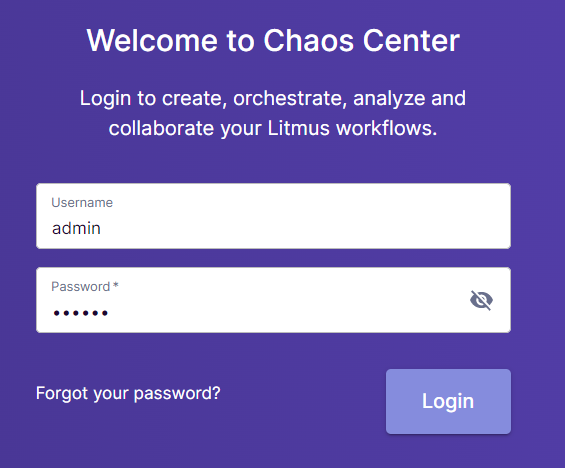
\includegraphics[scale=.5]{img/chaoscenter-login.png}
    \caption{login Litmus ChaosCenter}
\end{figure}

Nu de accountactivatie afgerond is zal men heel wat extra pods terugvinden in de namespace litmus. Dit kan men controleren door in de terminal het commando {\bf kubectl get pods -n litmus} uit te voeren. Een eerder gecreëerde cluster waarbij de resources per node te beperkt waren zorgde hier echter voor een falende pod genaamd 'event-tracker-[...]'. Deze pod bleef de status Pending behouden en door de pod te beschrijven via commando {\bf kubectl describe pod event-tracker-[...] -n litmus} kon onderaan bij Events te zien zijn dat onvoldoende CPU de oorzaak was. (zie onderstaande output)
 
\begin{lstlisting}[language=bash]
-- voorgaande output weggelaten --
-- volgende output ingekort     --
Events:
Type     Reason       From        Message
----     ------       ----        -------
Warning  Failed...    scheduler   0/3 nodes are available
                                  : 3 Insufficient cpu.
\end{lstlisting}
 
Vandaar bij voorgaand hoofdstuk in sectie \ref {sec:cloudclustersetup} het nodige belang gehecht werd aan voldoende resources toe te wijzen aan de nodes in de cluster. Volgende output toont aan dat de autoscaling configureren zijn nut bewees bij het herinstalleren van Litmus: 

\begin{lstlisting}[language=bash]
-- voorgaande output weggelaten --
-- volgende output ingekort     --
Events:
Type     Reason        From        Message
----     ------        ----        -------
Warning  Failed...     scheduler   0/3 nodes are available: 
                                   3 Insufficient cpu
Normal   Scheduled     scheduler   Successfully assigned ... 
Normal   Triggered...  autoscaler  pod triggered scale-up: 
                                   3 -> 4 (max: 6)
\end{lstlisting}

\subsection{Litmus experimenten uitvoeren via de terminal}

Vooraleer men experimenten kan uitvoeren moet men eerst volgende Litmus concepten begrijpen:
\begin{itemize}
    \item {\bf Chaos Experiment:} De generieke low-level code van een experiment waar men niks hoeft in te wijzigen.
    \item {\bf Chaos Engine:} De parameters waarmee men een experiment specifiek gaat richten naar een bepaalde applicatie/pod/... m.a.w. de connectie tussen applicatie en ChaosExperiment die men via een YAML-definitie configureert.
    \item {\bf Chaos Result:} Het resultaat van de uitvoer van een experiment. 
\end{itemize} 
 
Eerst zal in volgende subsecties een theoretische benadering geformuleerd worden hoe men een experiment dient op te zetten om uitgevoerd te worden via de terminal. Nadien wordt beschreven hoe het eerste experiment pod-delete opgezet kan worden. Vervolgens kan men nog een aantal andere uitgevoerde experimenten via de terminal terugvinden, alvorens over te gaan tot het uitvoeren van experimenten via de browser m.b.v. Litmus ChaosCenter.
 
\subsubsection{Experimenten installeren op het systeem}
\label{subsec:experimenteninstalleren}

Een experiment uit bovenstaande concept Chaos Experiment wordt bewaard in de Litmus Chaos Hub.  
Alle mogelijke Litmus experimenten kan men hier terugvinden, geklasseerd in verschillende categorieën. \autocite{ChaosHub2022} 

Men dient eerst de nodige categorie van experimenten te installeren in dezelfde namespace(s) van de demo-applicatie(s). De experimenten die via de terminal uitgevoerd worden vallen allen onder categorie {\bf generic/all-experiments}. \newline Om deze experimenten te installeren voert men volgend commando uit voor zowel de namespaces demoapp1 en demoapp2:
\begin{lstlisting}[language=bash]
$ kubectl apply -f \
https://hub.litmuschaos.io/api/chaos/2.7.0?file=charts/generic\
/experiments.yaml -n demoapp[1 en 2]
\end{lstlisting}

\subsubsection{Permissies van een experiment instellen}

Het uitvoeren van deze experimenten moet eerst voorafgegaan worden door de nodige permissies te configureren via {\bf Role Based Access Control (RBAC)}. Hierdoor verkrijgt het later beschreven experiment in de ChaosEngine de toestemming om uitgevoerd te worden binnen een bepaalde namespace. Permissies configureert men bij elk experiment wanneer men dit via de terminal uitvoert. 

Een vooraf gedefinieerde RBAC-configuratie per experiment kan men terugvinden via volgende link: \url{https://litmuschaos.github.io/litmus/experiments/categories/contents/}

De YAML-definitie in sectie {\bf Minimal RBAC configuration} slaat men op in een bestand onder een nieuw gecreëerde subdirectory (bv. serviceaccounts) in de alreeds bestaande directory litmus-experiments. Men hoeft enkel nog de waarde van elke parameter 'namespace' in dit bestand aanpassen naar de naam van de namespace waarin het experiment uitgevoerd wordt m.a.w. de namespace demoapp1 of demoapp2. \newline Via commando {\bf kubectl apply -f [bestand].yaml} maakt men vervolgens de nodige bestanden aan om de permissies te activeren.  

\subsubsection{Een ChaosEngine definiëren}

Nu de nodige permissies ingesteld zijn kan men een ChaosEngine definiëren waarin de link wordt gelegd naar het ChaosExperiment. Ook deze definitie kan men terugvinden in eerder vermelde link, in de sectie {\bf Experiment Examples}. Kopieer ook hier de inhoud en sla deze op in een nieuw bestand in de directory litmus-experiments. \autocite{Experiments2022}. 

Men zal zien dat in de ChaosEngine definitie de ServiceAccount aangesproken wordt. De parameter jobCleanUpPolicy zal er voor zorgen dat de 'helper pods' die Litmus lanceert tijdens het experiment terug verwijderd zullen worden na afloop.

Alle mogelijke parameters in aanvulling van een experiment kan men terugvinden in de sectie {\bf Experiment tunables}. Zo kan men o.a. beslissen via parameter CHAOS\textunderscore INTERVAL een experiment in iteraties uit te voeren, via parameter PODS\textunderscore AFFECTED\textunderscore PERC het percentage getroffen pods in te stellen ... 

\subsubsection{Een experiment uitvoeren}
\label{subsec:experimentuitvoeren}
Vervolgens is men klaar om een experiment uit te voeren. Dit kan men doen via commando {\bf kubectl apply -f [experiment-naam].yaml}. Dit commando zal géén output genereren. 

Tijdens de uitvoer kan men via de UI monitoring tool k9s het experiment live opvolgen. Hierin zal men eveneens zien dat in de demoapp[1/2] namespace tijdelijke helper pods gelanceerd worden om de uitvoer van het experiment te faciliteren. 

Enkele handige commando's om de uitvoer tijdens-, of het resultaat na een experiment te controleren zijn:
\begin{lstlisting}[language=bash]
# ChaosEngine object(en) oplijsten
$ kubectl get chaosengine -n demoapp[1 of 2]

# Het verloop van experiment tonen door het 
# ChaosEngine object te beschrijven
$ kubectl describe chaosengine [chaosengine] -n demoapp[1 of 2]

# ChaosResult object(en) oplijsten
$ kubectl get chaosresult -n demoapp[1/2]

# Het resultaat van experiment tonen door het 
# ChaosResult object te beschrijven
$ kubectl describe chaosresult [chaosresult] -n demoapp[1 of 2]
\end{lstlisting}

\subsection{Experiment 1: Nginx pod delete}

Bovenstaande theoretische benadering hoe men m.b.v. Litmus een experiment kan opzetten via de terminal zal in dit hoofdstuk omgezet worden naar de praktijk. Het eerste experiment die aan bod komt is het vernietigen van een Nginx pod in de namespace demoapp1. In deze namespace is ook een Deployment met Apache pods actief, die gevrijwaard zal blijven van de impact van dit experiment door dit zorgvuldig te configureren in de ChaosEngine definitie. 

De bedoeling van dit experiment is aantonen dat een pod vernietigen in Kubernetes opgevangen wordt door de ReplicaSet die bij een Deployment hoort. Deze zal er steeds voor zorgen dat het gewenste aantal pods van een Deployment verzekerd wordt.    

De nodige experimenten, geïnstalleerd in \ref{subsec:experimenteninstalleren} zijn alreeds aanwezig zowel in de namespace demoapp1 als demoapp2.
  
Via volgend stappenplan stelt men de permissies van het eerste pod-delete experiment en creëert men een ChaosEngine waarmee het experiment kan uitgevoerd worden: 
\begin{enumerate}
    \item Open volgende link via de browser: \url{https://litmuschaos.github.io/litmus/experiments/categories/contents/} 
    \item Ga in het linkermenu via de dropdownlist Kubernetes - Generic - Pod Chaos naar het experiment {\bf Pod Delete}. Daar vindt men de beschrijving en configuratie van dit experiment.
    \item Kopieer de YAML-definitie in sectie {\bf Minimal RBAC configuration}
    \item Ga naar de subdirectory /litmus-experiments/servicaccounts/
    \item Maak een nieuwe file pod-delete-sa.yaml aan en kleef de inhoud uit voorgaande stap hierin
    \item Verander bij elke parameter 'namespace:' de waarde default naar demoapp1, en sla vervolgens op.
    \item Voer het bestand uit via commando {\bf kubectl apply -f pod-delete-sa.yaml}. Dit zal volgende output genereren:
\begin{lstlisting}[language=bash]    
serviceaccount/pod-delete-sa created
role.rbac.authorization.k8s.io/pod-delete-sa created
rolebinding.rbac.authorization.k8s.io/pod-delete-sa created
\end{lstlisting}
    \item Herhaal bovenstaande stappen 1 en 2. Ga naar sectie {\bf Experiment Examples} en kopieer de inhoud van dit bestand.
    \item Maak een YAML-bestand aan in de directory litmus-experiments en noem dit bv. nginx-pod-kill.yaml
    \item Kleef de inhoud uit sectie {\bf Experiment Examples} in dit YAML-bestand en wijzig  de waarde van parameters namespace naar demoapp1, en applabel naar app=nginx, zodat het experiment specifiek gericht wordt op de nginx pods van de demo-applicatie in namespace demoapp1.
    \item Sla het bestand op en voer het experiment uit via {\bf kubectl apply -f nginx-pod-kill.yaml}
    \item Volg het experiment op via k9s of via commando's uit subsectie \ref{subsec:experimentuitvoeren}: Een experiment uitvoeren.
\end{enumerate}

